\renewcommand{\prechaptername}{付録}
\renewcommand{\postchaptername}{}
\renewcommand{\thechapter}{\Alph{chapter}}
\setcounter{chapter}{0}

\chapter{タイミング較正結果}
\thispagestyle{empty}
\label{app:app1}
TGC~検出器のすべてのチェンバーにおけるタイミング較正の結果を示す。タイミングの評価には\equref{eq:timing}のパラメータを使用している。タイミング較正後のシミュレーションが~Run~2~の実験データをよく再現していることが分かる。
\figref{fig:timingPlotCompWireM1}、\figref{fig:timingPlotCompWireM2}、\figref{fig:timingPlotCompWireM3}、\figref{fig:timingPlotCompWireEIFI}はそれぞれ~M1、M2、M3、EIFI~のワイヤーチャンネルにおけるタイミング分布、
\figref{fig:timingPlotCompStripM1}、\figref{fig:timingPlotCompStripM2}、\figref{fig:timingPlotCompStripM3}、\figref{fig:timingPlotCompStripEIFI}はそれぞれ~M1、M2、M3、EIFI~のストリップチャンネルにおけるタイミング分布を示す。

    \begin{figure}[htbp]
    		\begin{minipage}{0.49\hsize}
			\centering
			\includegraphics[width=\textwidth,page=2]{img/pdf5/master_timingplot_comp.pdf}
			\end{minipage}
			\begin{minipage}{0.49\hsize}
			\centering
			\includegraphics[width=\textwidth,page=4]{img/pdf5/master_timingplot_comp.pdf}
			\end{minipage}\\
			\begin{minipage}{0.49\hsize}
			\centering
			\includegraphics[width=\textwidth,page=6]{img/pdf5/master_timingplot_comp.pdf}
			\end{minipage}
			\begin{minipage}{0.49\hsize}
			\centering
			\includegraphics[width=\textwidth,page=8]{img/pdf5/master_timingplot_comp.pdf}
			\end{minipage}\\
			\begin{minipage}{0.49\hsize}
			\centering
			\includegraphics[width=\textwidth,page=10]{img/pdf5/master_timingplot_comp.pdf}
			\end{minipage}
		\caption[M1~ワイヤーチャンネルにおけるタイミングパラメータを用いた~TGC~の評価。]{M1~ワイヤーチャンネルにおけるタイミングパラメータを用いた~TGC~の評価。橙色(■)、緑色(●)、青色(▲)はそれぞれRun~2~データ、改良後のシミュレーション、改良前のシミュレーションを表している。各プロットにチェンバーの名称を示している。}
		\label{fig:timingPlotCompWireM1}
	\end{figure}
	
	\begin{figure}[htbp]
         \begin{minipage}{0.49\hsize}
        \centering
        \includegraphics[width=\textwidth,page=12]{img/pdf5/master_timingplot_comp.pdf}
		\end{minipage}
		\begin{minipage}{0.49\hsize}
		\centering
		\includegraphics[width=\textwidth,page=14]{img/pdf5/master_timingplot_comp.pdf}
		\end{minipage}\\
		\begin{minipage}{0.49\hsize}
		\centering
		\includegraphics[width=\textwidth,page=16]{img/pdf5/master_timingplot_comp.pdf}
		\end{minipage}
		\begin{minipage}{0.49\hsize}
		\centering
		\includegraphics[width=\textwidth,page=18]{img/pdf5/master_timingplot_comp.pdf}
	    \end{minipage}\\
	    \begin{minipage}{0.49\hsize}
		\centering
		\includegraphics[width=\textwidth,page=20]{img/pdf5/master_timingplot_comp.pdf}
		\end{minipage}
		\begin{minipage}{0.49\hsize}
		\centering
		\includegraphics[width=\textwidth,page=22]{img/pdf5/master_timingplot_comp.pdf}
		\end{minipage}
		\caption[M2~ワイヤーチャンネルにおけるタイミングパラメータを用いた~TGC~の評価。]{M2~ワイヤーチャンネルにおけるタイミングパラメータを用いた~TGC~の評価。橙色(■)、緑色(●)、青色(▲)はそれぞれRun~2~データ、改良後のシミュレーション、改良前のシミュレーションを表している。各プロットにチェンバーの名称を示している。}
		\label{fig:timingPlotCompWireM2}
	\end{figure}
\begin{figure}[htbp]
		
	
			\begin{minipage}{0.49\hsize}
			\centering
			\includegraphics[width=\textwidth,page=24]{img/pdf5/master_timingplot_comp.pdf}
			\end{minipage}
			\begin{minipage}{0.49\hsize}
			\centering
			\includegraphics[width=\textwidth,page=26]{img/pdf5/master_timingplot_comp.pdf}
			\end{minipage}\\
			\begin{minipage}{0.49\hsize}
			\centering
			\includegraphics[width=\textwidth,page=28]{img/pdf5/master_timingplot_comp.pdf}
			\end{minipage}
			\begin{minipage}{0.49\hsize}
			\centering
			\includegraphics[width=\textwidth,page=30]{img/pdf5/master_timingplot_comp.pdf}
			\end{minipage}\\
			\begin{minipage}{0.49\hsize}
			\centering
			\includegraphics[width=\textwidth,page=32]{img/pdf5/master_timingplot_comp.pdf}
			\end{minipage}
			\begin{minipage}{0.49\hsize}
			\centering
			\includegraphics[width=\textwidth,page=34]{img/pdf5/master_timingplot_comp.pdf}
			\end{minipage}
			\caption[M3~ワイヤーチャンネルにおけるタイミングパラメータを用いた~TGC~の評価。]{M3~ワイヤーチャンネルにおけるタイミングパラメータを用いた~TGC~の評価。橙色(■)、緑色(●)、青色(▲)はそれぞれRun~2~データ、改良後のシミュレーション、改良前のシミュレーションを表している。各プロットにチェンバーの名称を示している。}
		\label{fig:timingPlotCompWireM3}
	\end{figure}
	
\begin{figure}[htbp]
			\begin{minipage}{0.49\hsize}
			\centering
			\includegraphics[width=\textwidth,page=36]{img/pdf5/master_timingplot_comp.pdf}
			\end{minipage}
			\begin{minipage}{0.49\hsize}
			\centering
			\includegraphics[width=\textwidth,page=38]{img/pdf5/master_timingplot_comp.pdf}
			\end{minipage}\\
			\begin{minipage}{0.49\hsize}
			\centering
			\includegraphics[width=\textwidth,page=40]{img/pdf5/master_timingplot_comp.pdf}
			\end{minipage}
			\begin{minipage}{0.49\hsize}
			\centering
			\includegraphics[width=\textwidth,page=42]{img/pdf5/master_timingplot_comp.pdf}
			\end{minipage}
		\caption[EIFI~ワイヤーチャンネルにおけるタイミングパラメータを用いた~TGC~の評価。]{EIFI~ワイヤーチャンネルにおけるタイミングパラメータを用いた~TGC~の評価。橙色(■)、緑色(●)、青色(▲)はそれぞれRun~2~データ、改良後のシミュレーション、改良前のシミュレーションを表している。各プロットにチェンバーの名称を示している。}
		\label{fig:timingPlotCompWireEIFI}
	\end{figure}
    
    \begin{figure}[htbp]
			\begin{minipage}{0.49\hsize}
			\centering
			\includegraphics[width=\textwidth,page=3]{img/pdf5/master_timingplot_comp.pdf}
    		\end{minipage}
			\begin{minipage}{0.49\hsize}
			\centering
			\includegraphics[width=\textwidth,page=5]{img/pdf5/master_timingplot_comp.pdf}
			\end{minipage}\\
			\begin{minipage}{0.49\hsize}
			\centering
			\includegraphics[width=\textwidth,page=7]{img/pdf5/master_timingplot_comp.pdf}
			\end{minipage}
			\begin{minipage}{0.49\hsize}
			\centering
			\includegraphics[width=\textwidth,page=9]{img/pdf5/master_timingplot_comp.pdf}
			\end{minipage}\\
			\begin{minipage}{0.49\hsize}
			\centering
			\includegraphics[width=\textwidth,page=11]{img/pdf5/master_timingplot_comp.pdf}
			\end{minipage}
		\caption[M1~ストリップチャンネルにおけるタイミングパラメータを用いた~TGC~の評価。]{M1~ストリップチャンネルにおけるタイミングパラメータを用いた~TGC~の評価。橙色(■)、緑色(●)、青色(▲)はそれぞれRun~2~データ、改良後のシミュレーション、改良前のシミュレーションを表している。各プロットにチェンバーの名称を示している。}
		\label{fig:timingPlotCompStripM1}
	\end{figure}
	
	\begin{figure}[htbp]
            \begin{minipage}{0.49\hsize}
        	\centering
			\includegraphics[width=\textwidth,page=13]{img/pdf5/master_timingplot_comp.pdf}
			\end{minipage}
			\begin{minipage}{0.49\hsize}
			\centering
			\includegraphics[width=\textwidth,page=15]{img/pdf5/master_timingplot_comp.pdf}
			\end{minipage}\\
			\begin{minipage}{0.49\hsize}
			\centering
			\includegraphics[width=\textwidth,page=17]{img/pdf5/master_timingplot_comp.pdf}
			\end{minipage}
			\begin{minipage}{0.49\hsize}
			\centering
			\includegraphics[width=\textwidth,page=19]{img/pdf5/master_timingplot_comp.pdf}
			\end{minipage}\\
			\begin{minipage}{0.49\hsize}
			\centering
			\includegraphics[width=\textwidth,page=21]{img/pdf5/master_timingplot_comp.pdf}
			\end{minipage}
			\begin{minipage}{0.49\hsize}
			\centering
			\includegraphics[width=\textwidth,page=23]{img/pdf5/master_timingplot_comp.pdf}
			\end{minipage}
		\caption[M2~ストリップチャンネルにおけるタイミングパラメータを用いた~TGC~の評価。]{M2~ストリップチャンネルにおけるタイミングパラメータを用いた~TGC~の評価。橙色(■)、緑色(●)、青色(▲)はそれぞれRun~2~データ、改良後のシミュレーション、改良前のシミュレーションを表している。各プロットにチェンバーの名称を示している。}
		\label{fig:timingPlotCompStripM2}
	\end{figure}
	
	\begin{figure}[htbp]
			\begin{minipage}{0.49\hsize}
			\centering
			\includegraphics[width=\textwidth,page=25]{img/pdf5/master_timingplot_comp.pdf}
			\end{minipage}
			\begin{minipage}{0.49\hsize}
			\centering
			\includegraphics[width=\textwidth,page=27]{img/pdf5/master_timingplot_comp.pdf}
			\end{minipage}\\
			\begin{minipage}{0.49\hsize}
			\centering
			\includegraphics[width=\textwidth,page=29]{img/pdf5/master_timingplot_comp.pdf}
			\end{minipage}
			\begin{minipage}{0.49\hsize}
			\centering
			\includegraphics[width=\textwidth,page=31]{img/pdf5/master_timingplot_comp.pdf}
			\end{minipage}\\
			\begin{minipage}{0.49\hsize}
			\centering
			\includegraphics[width=\textwidth,page=33]{img/pdf5/master_timingplot_comp.pdf}
			\end{minipage}
			\begin{minipage}{0.49\hsize}
			\centering
			\includegraphics[width=\textwidth,page=35]{img/pdf5/master_timingplot_comp.pdf}
			\end{minipage}
		\caption[M3~ストリップチャンネルにおけるタイミングパラメータを用いた~TGC~の評価。]{M3~ストリップチャンネルにおけるタイミングパラメータを用いた~TGC~の評価。橙色(■)、緑色(●)、青色(▲)はそれぞれRun~2~データ、改良後のシミュレーション、改良前のシミュレーションを表している。各プロットにチェンバーの名称を示している。}
		\label{fig:timingPlotCompStripM3}
	\end{figure}
	
	\begin{figure}[htbp]
			\begin{minipage}{0.49\hsize}
			\centering
			\includegraphics[width=\textwidth,page=37]{img/pdf5/master_timingplot_comp.pdf}
			\end{minipage}
			\begin{minipage}{0.49\hsize}
			\centering
			\includegraphics[width=\textwidth,page=39]{img/pdf5/master_timingplot_comp.pdf}
			\end{minipage}\\
			\begin{minipage}{0.49\hsize}
			\centering
			\includegraphics[width=\textwidth,page=41]{img/pdf5/master_timingplot_comp.pdf}
			\end{minipage}
			\begin{minipage}{0.49\hsize}
			\centering
			\includegraphics[width=\textwidth,page=43]{img/pdf5/master_timingplot_comp.pdf}
			\end{minipage}
		\caption[EIFI~ストリップチャンネルにおけるタイミングパラメータを用いた~TGC~の評価。]{EIFI~ストリップチャンネルにおけるタイミングパラメータを用いた~TGC~の評価。橙色(■)、緑色(●)、青色(▲)はそれぞれRun~2~データ、改良後のシミュレーション、改良前のシミュレーションを表している。各プロットにチェンバーの名称を示している。}
		\label{fig:timingPlotCompStripEIFI}
	\end{figure}
	